%% ----------------------------------------------------------------
%% Thesis.tex -- main
%% ---------------------------------------------------------------- 

\documentclass[a4paper, 10pt, oneside]{memoir}
\usepackage{basilea}
\usepackage{geometry}% http://ctan.org/pkg/geometry
\usepackage{array}% http://ctan.org/pkg/
%\usepackage{ccaption}% http://ctan.org/pkg/ccaption
\usepackage[math]{cellspace}
\usepackage{mathtools}
\usepackage{textcomp} % to write the degre sign: °
\usepackage{lipsum}
\usepackage{placeins}
\usepackage{pdfpages}
\usepackage{pgfplots}
\pgfplotsset{width=9cm,compat=1.9}
\cellspacetoplimit 4pt
\cellspacebottomlimit 4pt

\renewcommand\todo[0]{\textcolor{red}{TODO!}}

%% ----------------------------------------------------------------

\title				{An Empirical Comparison of Deep Learning and 3DMM-based Approaches for Facial Occlusion Segmentation}
\thesistype			{Bachelor-Thesis}

\department 		{Department of Mathematics and Computer Science}
\faculty			{Natural Science Faculty of the University of Basel}
\research		    {Computer Graphics and Vision (Gravis) \\ http://gravis.dmi.unibas.ch/}

\examiner    		{Prof. Dr. Thomas Vetter}
\supervisor  		{Dr. Adam Kortylewski}

\authors     		{Elias Arnold}
\email				{elias.arnold@stud.unibas.ch}
\immatriculnr		{14-930-770}

\date				{10.08.2018}

% switch here for the german logo to logo-de
\ulogo				{Template/logo-en} 


%% ----------------------------------------------------------------
\begin{document}

% for english use \selectlanguage{english}, for german use \selectlanguage{ngerman}
\selectlanguage{english}

\thesisfront
\maketitle
\pagestyle{thesis}
%% ----------------------------------------------------------------
\chapter{Acknowledgments}
I would like to thank Dr. Adam Kortylewski as my main supervisor for the guidance and insight through the work and  writing of this thesis. In addition, I would like to thank Prof.  Dr.  Vetter for the possibility to write this thesis in his
research group.
%% ----------------------------------------------------------------
\chapter{Abstract}
This thesis evaluates a pretrained Fully Convolutional Network to segment images into face and non-face region. The result of this segmentation is a binary encoded image. Such a segmentation can be used to limit an algorithm to a specific image region, so that not the entire image has to be scanned by the algorithm. \\ \\

\lipsum[1-3]
%% ----------------------------------------------------------------
\thesistoc
%% ----------------------------------------------------------------
%\thesisnomencl
%% ----------------------------------------------------------------
\thesismain
\chapter{Introduction}
Fitting is the process of generating a 3D model of a face from a 2D image. There are different approaches on how to do that. The gravis group of the University of Basel has developed an MCMC (Markov Chain Monte Carlo) algorithm that makes random changes to a 3DMM (3D Morphable Model) and accepts the proposal face whenever the new 3D face has a greater probability than the previous one. For this Thesis, we use the popular Basel Face Model 2017 \cite{BFM2017}. That the algorithm can determine the likelihood of a 3D facial proposal relative to a given 2D face, the algoritm's evaluator needs to now, which pixels to include in the probability calculation. Therefore we have to label each pixel if it's part of the face which should be regarded by the evaluator, or if it's background and hsn't any importance for the construction of the 3D Model. Nirkin et al \cite{nirkin2018_faceswap} claim, that this is possible with a standart fully convolutional network.\\ 
\\
The idea of Artificial Neural Networks was heavily influenced by biology. They consist of a variety of neurons which are grouped in layers. The way each neuron works is very simple. It takes multiple inputs of varying strength from other neurons, sums them up and decides depending on the sum whether it should send a stimulus itself and if so, in which strength. Each layer is somehow connected to the next layer. Some layers are fully connected (each neuron of a layer is connected to every other neuron in the next layer) while others are convolutional. Convolutional means that a neuron only gets input of its neighbors in a previous layer. There are many different architectures which mainly differ in the number of layers, number of neurons per layer and the interconnectivity of the neurons. A classical Convolutional Neural Network (CNN) has the following structure:
\begin{figure}
	\centering
	\includegraphics[width=1\linewidth]{Figures/chap1/classicalCNN.JPG}
	\caption{In the lower-left corner, you see the 16 layers of the VGG16-FCN. Each Max-Pooling layer cuts the input image size in half. In the top-right, you can see the meaning of the '8s' term of the FCN-Name. It means that the resulting image has to be 8x upsampled, to get an image which is in size equal to the input image (which means we have four pooling-layers)}
	\label{fig:test1}
\end{figure}\\
In 1943 Warren McCulloch and Walter Pitts \cite{mcculloch} showed that even simple networks of this kind can simulate every possible logic-gate. For this they used a neuron model that consisted of simple logic gates and could process only binary input and output signals.

\begin{figure}
	\centering
	\includegraphics[width=1\linewidth]{Figures/chap1/bio_vs_arti_neuron.png}
	\caption[Caption for LOF]{The left-hand side of the image \footnotemark shows a Biological Neuron. It is a nerve cell that occurs in almost every animal. On the right-hand side is On the right is an artificial neuron. It sums up the stimuli of the previous neurons, applies an activation function to this sum and forwards the output of this function itself}
	\label{fig:test1}
\end{figure}

\footnotetext{Source: Google.com}

\begin{figure}
	\centering
	\includegraphics[width=\linewidth]{Figures/chap1/ActivFunctionsSimpleANN.png}
	\caption{\todo}
	\label{fig:test1}
\end{figure}

\section{The network used}
\label{sec:theFCN}
For this thesis, we used a pretrained fully convolutional network from \cite{nirkin2018_faceswap}. A Fully Convolutional Network (often called: FCN) is basically a CNN but with a modified architecture. An FCN doesn't have the fully connected layers usually found at the end of an CNN. These layers would enable the Network to make decisions based on global information. Aa CNN can for example be used for classification. But for image analysis we want local information of the input image (we don't want to know if there is a face in the image, but where the face is in the image). Therefore a FCN uses only convolutional and pooling layers. In the whole Fully Convolutional Network only the following structure is repeated: One or more convolution layers and a pooling layer which downsamples the picture. This constellation is repeated several times.\\
\\
The assembly of our network used for this thesis follows the FCN-8s-VGG architecture with extensions of \cite{jlong}. The first part 'FCN' stands for 'fully convolutional network', '8s' means that the result gets eight times upsampled (4 pooling layers) and 'VGG' means the popular 16-layer network used by Oxford's Visual Geometry Group \cite{ksimonyan}. The original task of the network was to find the name of an object in an input image. The network could distinguish between 1000 different objects. Each cell in the final Softmax-Layer (1*1000 in size) was a boolean variable for one specific object.

\begin{figure}
	\centering
	\includegraphics[width=1\linewidth]{Figures/fcn_1.png}
	\caption{In the lower-left corner, you see the 16 layers of the VGG16-FCN. Each Max-Pooling layer cuts the input image size in half. In the top-right, you can see the meaning of the '8s' term of the FCN-Name. It means that the resulting image has to be 8x upsampled, to get an image which is in size equal to the input image (which means we have four pooling-layers)}
	\label{fig:test1}
\end{figure}


\section{Related Work}
For our experiments we used a pretrained Fully Convolutional Network (FCN) of \cite{nirkin2018_faceswap}. They showed that even with a widespread network, you can do good segmentation and that the network does not have to be specially tailored to the future purpose. But the network must have been trained with a large enough data set. For more details about the used FCN and the architecture see section \ref{sec:theFCN}. They used the FCN for intra- and intersubject face swapping on the Labeled Faces in the Wild (LFW) data set and showed that intra-subject swapped faces remain as recognizable as before the swap and that in the intersubject version better face swapping  leads to less perceptibility.\\
\\
They used a semi-supervised approach to produce training data in order to train the FCN. To produce large quantities of them, they used 2'043 face videos of the IARPA Janus CS2 dataset. To avoid searching for the face in every frame of the video they used motion queues which tracked the face based on an initial segmentation based on \cite{grundmann} which enriched their trainingset to 9'818 images. To enlarge the collection of images, they rendered 3D Shapes of of various objects (e.g. sunglasses, hands) into existing images. Each occlusion added 9'500 images to their trainingset.\\
\\
The gravis group of the University of Basel developped "Occlusion Aware 3D Morphable Models" \cite{egger_paper}. These Methods use an iterative approach to generate the z-labels, namely to label each pixel wether it belogs to the face or is background. This approach can handle multiple labels and differentiate between multiple occlusion types. For example face specific ones (eg. beards, sunglasses) and background. For updating the z-labels they use an EM-like algorithm which classifies a pixel based on the probabilities for each possible label.  But for our experiments we limited ourselves to two. We only need to distinguish face (including skin and beard) and background.\\ 
\\
They used an EM-algorithm like method to solve two problems simultaneusly. In the E-steps they updated the z-labels and in the M-steps they updated the face parameters. Conventional approaches often fail on important parts of the face such as the eyes, eyebrows or the oral region because oftheyr strong variability in color and shape. The segmentation of \cite{egger_paper} also has difficulties with these aspects as Figure \ref{fig:iterations} shows.

% The source for this table was this post: https://stackoverflow.com/questions/2771856/centering-text-horizontally-and-vertically-in-latex
% To add padding for the cell contents: https://tex.stackexchange.com/questions/31672/column-and-row-padding-in-tables
\begin{figure}[h]
	\begin{center}
		\newcolumntype{C}{>{\centering\arraybackslash} m{3cm} }  %# New column type
		\begin{tabular}{SC|SC|SC|SC}
			 target image & initial segmentation & after 10 iterations & after 20 iterations\\ \hline
			\subfloat{\includegraphics[width=0.2\textwidth]{Figures/chap1/angie_original.png}} &
			\subfloat{\includegraphics[width=0.2\textwidth]{Figures/chap1/EGGER_Segmentation_Nr_0.png}} &
			\subfloat{\includegraphics[width=0.2\textwidth]{Figures/chap1/EGGER_Segmentation_Nr_9.png}} &
			\subfloat{\includegraphics[width=0.2\textwidth]{Figures/chap1/EGGER_Segmentation_Nr_19.png}} \\
		\end{tabular}
	\end{center}
	\caption{It's obvious that the initial segmentation doesn't include the whole face region. Striking in this sample image are not only the eyes as mentioned before but also the shadow of the nose, which is first segmented as a background. Only after a certain number of iterations these errors are partially recognized and provided with the correct label.}
	\label{fig:iterations}
\end{figure}

An approach using convolutional neural networks to segment occluded faces has already been described by \cite{SaitoEtAl}. The big difference to our approach is that multiple frames are needed for the final segmentation. An other approach of \cite{MorelForster} integrate occlusion into the fitting process to model an uncertainty. They use random forests to detect facial-occlusions by hair.

\begin{itemize}
	\item Work of Nirkin et al. (Their results)
	\item Summarize Paper: "Occlusion-aware 3D Morphable Models and..."
	\item Work of Saito et al.
	\ Work of Morel-Forster (2017)
\end{itemize}

\section{Expectations of the FCN}
Because \cite{nirkin2018_faceswap} trained the FCN on a very large and diverse dataset, we expect the network to perform well in the task of segmenting a face. They claim that a standart segmentation network is sufficient to segment as well as a network especially tailored for this task and outperforms state of the art methods for face segmentation. We create multiple synthetic faces and render various occlusions over them. We expect the FCN to do well on usual facial-occlusions (eg. hands, microphones).

	\begin{itemize}
		\item We expect the FCN to perform well of occlusions used for training, e.g. hands, microphones
		\item An FCN is known to be very fast, so we expect to speed up the fitting.
	\end{itemize}






\chapter{Evaluation}
\section{Evaluation on Datasets}
\label{sec:EvaluationOnDatasets} % Now, we can use "\autoref{sec:<my-label>}" to refer to this chapter
The face segmentation network was tested on two different datasets 1.) The Caltech occluded faces in the wild (COFW) and 2.) parts-labeled LFW Dataset of the University of Massachusetts.\\
\\
Nirkin et al. \cite{nirkin2018_faceswap} claim that both the face itself an the context of the face play an important role for the outcome of the segmentation. To measure this effect and reduce the impact of outliers, we repeat each experiment multiple times with a different face and a different backgroundimage. Within a dataset The face and the backgroundimage stay the same. For the results we use the average of all results.
\subsection{COFW}
Since on the COFW dataset, only landmarks and bounding-boxes are given, the segmentation had to be evaluated qualitatively. We weren't able to count the correctly labeled pixels of the with respect to a ground-truth mask. To increase the precision of the network, we cropped the images according to the provided bounding-boxes. Because the bounding-boxes were only inluding the eyes and the mouth of the subject, we had to add an offset which was optically determined. Therefore, we measured the quality of the neural network only qualitatively. Nevertheless, we tried to reconstruct the graphic on Nirkis[1] github-page.
\begin{figure}[h]
	\centering
	\includegraphics[width=.75\textwidth]{Figures/myMatrix.jpg}
	\caption{18 images of the COFW Dataset overlayd with the FCN output (in red). The given box was extended upwards by 80\%, to the right and left it was 55\% and downwards t was 5\%.}
	\label{figure2}
\end{figure}

\newpage

\subsection{Parts-LFW}
In the Parts-LFW Database, we had a ground-truth mask for every image. Unfortunately, the FCN of Nirkin[1] segmented facial hair and on the masks, facial hair was excluded. So we had to manually remove these images. To reduce the effort, we took the Parts-LFT Validation set containing 500 images. After removing the ones with a beard or mustache, we were left with 447 images. The results are summarized in the following table:\\
%\vspace{.5cm}\\
\begin{figure}
\begin{center}
\begin{tabular}{l|l} \hline
	false-positives (hair) & 7.04\%\\ \hline
	false-positives (background) & 0.68\%\\ \hline
	right-segmentations & 85.87\%\\ \hline
	right non-sementations & 99.32\% \\ \hline
\end{tabular}
\end{center}
\caption{\todo} 
\label{fig:Parts-LFW}
\end{figure}
%\vspace{.5cm}

\section{Evaluation on synthetic-data}
In order to evaluate the FCN on synthetic-data, we used the Parametric-Face-Image-Generator of \cite{parametric} to produce images of a random face in a given pose. We extended the software so that it now renders occlusions over the face. Further, the Parametric-Face-Image-Generator now produces a Ground-Truth-Mask, which classifies every pixel either as part of the face or as non-face.

\subsection{Dpendence of the Euler angles}
Because we can now create synthetic face images in any desired pose, we first wanted to find out the accuracy of segmenting the FCN for the angles: Yaw, Roll, and Pitch. In order to do that, we produced with the tool of \cite{parametric} 101 face images for every angle from $-50$\textdegree to $50$\textdegree. In every picture, the face is turned one degree further. We evaluated each angle itself and every possible combination of the angles in order to to create a hierarchy under the angles:

\begin{figure}[h]
	\centering
	\includegraphics[width=\textwidth]{Figures/evaluation_angles.png}
	\label{fig:evaluation_angles}
	\caption{In the plots on the top row we see the segmetation accuracy in percent (on the y-axis) for every single image (with face angle from $-50$\textdegree to $50$\textdegree on the x-axis). The point cloud is approximated by a quadratic function via a least squares fit (red curve / $f(x)$). The first parameter of this function determines the opening angle ($p_1$). From these graphs we can conclude that the roll angle is the most relevant for the FCN. The pitch-angle is less important and that the accuracy of the FCN is still good even with hith angles (least important). In the bottom row the colors indicate the segmentation accuracy. The brighter the color, the better the segmentation. In every plot, there is a cluster of high accuracy segmentations centered in the origin. The angle on whose axis the cluster has the lesser extent is the more important of the two. We call an angle important, when a small change of this angle leads to a failure of the FCN. }
\end{figure}

\subsection{random boxes as occlusions}
With the parametric-face-image-generator of \cite{parametric}, we produced about 5.2 thousand images of Which for every angle from $-40$\textdegree to $40$\textdegree  include 100 images of 5 different faces with 20 different occlusion levels. In the given table (Figure \ref{fig:angle_table}) all provided images show a face, from which 20\% of the pixels are occluded by a randomly colored box. We can optically verify, that 1) the yaw angle, despite the occluding box, hasn't much of an effect. 2.) In both situations, -40 and 40, of the roll angle, the result is not satisfying. 3.) In the third column, the segmentation with a negative pitch angle is much worse than with a positive one! Note that the results for each grid cell in figure \ref{fig:occVal40} is based on 5 segmentations (5200 images over all)!\\

% The source for this table was this post: https://stackoverflow.com/questions/2771856/centering-text-horizontally-and-vertically-in-latex
% To add padding for the cell contents: https://tex.stackexchange.com/questions/31672/column-and-row-padding-in-tables
\begin{figure}[h]
	\begin{center}
		\newcolumntype{C}{>{\centering\arraybackslash} m{2cm} }  %# New column type
		\begin{tabular}{m{1cm}|SC|SC|SC}
			& yaw & roll & pitch\\ \hline
			-40 & \subfloat{\includegraphics[width=0.1\textwidth]{Figures/-40_0_0_occVal_20.png}} &
			\subfloat{\includegraphics[width=0.1\textwidth]{Figures/0_0_-40_occVal_20.png}} &
			\subfloat{\includegraphics[width=0.1\textwidth]{Figures/0_-40_0_occVal_20.png}} \\ \hline
			40 & \subfloat{\includegraphics[width=0.1\textwidth]{Figures/40_0_0_occVal_20.png}} &
			\subfloat{\includegraphics[width=0.1\textwidth]{Figures/0_0_40_occVal_20.png}} &
			\subfloat{\includegraphics[width=0.1\textwidth]{Figures/0_40_0_occVal_20.png}} \\
		\end{tabular}
	\end{center}
	\caption{asdfasdf\todo}
	\label{fig:angle_table}
\end{figure}
Although boxes as occlusions are very simpley and we're in control of the rectangle's size, we can occlude a given amount of the face region with this method, but in practice, exact rectangles are very rare. That's why we left it with the rectangles and used real-world objects (e.g. hands, microphones or sunglasses) as synthetic occlusions. Unlike Nirkin[1], we didn't use the landmarks of the face for this task. We placed them randomly on the image instead. Thats the reason why we use a second plot to show the percentage of occluded face pixels in the following.

\begin{figure}[h]
	\centering
	\includegraphics[width=\textwidth]{Figures/occVal_angles.png}
	\caption{The color of each grid cell indicates the accuracy of the segmentation of the FCN on a set of faces turned by the corresponding angle and occluded with a square, so that the corresponding amount of the face is masked. The brighter the color, the better the segmentation. On each plot, we would expect to see a triangle pointing to the right. This means that the combination of a large angle and a large occlusion make the face even more unsegmentable.}
	\label{fig:occVal40}
\end{figure}
We see that the segmentation is very sensitive to roll-angles and the FCN is not trained to segment faces in every rotation! Surprisingly, the yaw angle plays a subordinate role here. The right most plot tells us, that the sign of the pitch angle plays a significant role! Since we aren't able to determine at which angles exactly the FCN begins to fail,we repeated the experiment with a higher angle range:\\

\begin{figure}[h!]
	\centering
	\includegraphics[width=\textwidth]{Figures/occVal_angles_90.png}
	\caption{This plot shows the outcome of a similar expreiment as snown in Figure \ref{fig:occVal40} with less resolution. All the angles (yaw, pitch and roll) range from $-90$\textdegree to $90$ \textdegree. The scale on the "\%-occlusion" stays the same as in Figure \ref{fig:occVal40} We can clearly see the limits of the FCN even with a occlusion of 2\%! Very interestig is the hard transition from good segmentations to bad segmentations in the two right plots.}
	\label{fig:occVal90}
\end{figure}

%\newpage
%
%\begin{figure}[t]
%	\contcaption{This plot shows the outcome of a similar experiment as shown in Figure \ref{figure5} with less resolution. All the angles (yaw, pitch and roll) range from -90 to 90 dergrees. The scale on the "\%-occlusion" stays the same as in Figure \ref{figure5} We can clearly see the limits of the FCN even with a occlusion of 2\%! Very interestig is the hard transition from good segmentations to bad segmentations in the two right plots.}% Continued caption
%\end{figure}

%In the new version of the parametric-face-image-generator the option "occlusionMode" can now be set to:
%\begin{itemize}
%	\item \textbf{"random"}: A randomly choosen occlusion image hides the picture in a random place.
%	\item \textbf{"box"}: Boxes, filled with either an arbitrary color or gaussian-white-noise hide the image.
%	\item \textbf{"box-whitenoise"}: Boxes, filled with gaussian-white-noise only.
%	\item \textbf{"eyes"}: Black boxes hiding the eyes on the face in the image.
%\end{itemize}
%In addition to the output Images, the parametric-face-image-generator now provides masks as well. They can be used as ground truth for the position of the face and te occlusion.
%\subsection{Sub-Section}
%
%\subsubsection{Sub-Sub-Section}
%
%\paragraph{Paragraph}
%
%\subparagraph{Even Sub-Paragraph}
%
%This is the body text. Make sure that when you reference anything you use labels and references. When you refer to anything, you normally capitalise the type of object you reference to, e.g. Section~\ref{sec:EvaluationOnDatasets} instead of section~\ref{sec:my-label}. You may also just use the \texttt{cref} command and it will generate the label, e.g., for \cref{sec:my-label}, we did not specify the word ``Section''.\cite{turing:1950}
%
%Hint: Try to structure your labels as it is done with \texttt{sec:my-label} and \texttt{fig:machine}, etc.
%
%
%
%\section{Equations}
%A Turing Machine is a 7-Tuple:
%\begin{equation}
%    M = \langle Q, \Gamma, b, \Sigma, \delta, q_0, F \rangle
%\end{equation}
%A Turing Machine is a 7-Tuple even if defined in the text, as in $M = \langle Q, \Gamma, b, \Sigma, \delta, q_0, F \rangle$.
%
%
%
%
%\section{Tables}
%Some tables can also be used as shown in Table~\ref{tab:table}\footnote{Table captions are normally above the table.}. Remember that tables might be positioned elsewhere in the document. You can force positioning by putting a \texttt{ht!} in the definition.
%
%\begin{table}[ht!]
%\centering
%\caption{Frequency of Paper Citations. By the way: Make sure to put the label always after the caption, otherwise \LaTeX{} might reference wrongly!}
%\begin{tabular}{lcl} \toprule
%Title&$f$&Comments\\ \midrule
%The chemical basis of morphogenesis & 7327 & \\ 
%On computable numbers, with an application to the ... & 6347 & Turing Machine\\
%Computing machinery and intelligence & 6130 & \\ \bottomrule
%\end{tabular}
%\label{tab:table}
%\end{table}
%
%
%
%
%\section{Figures}
%Figures are nice to show concepts visually. For organising well your thesis, put all figures in the Figures folder. Figure~\ref{fig:machine} shows how to insert an image into your document. Figure~\ref{fig:tm} references a figure with multiple sub-figures. \todoMissing{Description of figure.}
%
%\begin{figure}
%\centering
%\includegraphics[width=0.9\textwidth]{turingmachine}
%\caption{A Turing machine.}
%\label{fig:machine}
%\end{figure}
%
%
%\begin{figure}
%\centering
%\subbottom[Turing Machine 1]{\includegraphics[width=0.2\textwidth]{block}\label{fig:tm:tm1}}
%\subbottom[Turing Machine 2]{\includegraphics[width=0.2\textwidth]{block}\label{fig:tm:tm2}}
%\subbottom[Turing Machine 3]{\includegraphics[width=0.2\textwidth]{block}\label{fig:tm:tm3}}
%\subbottom[Turing Machine 4]{\includegraphics[width=0.2\textwidth]{block}\label{fig:tm:tm4}}
%\caption{Plots of four Turing machines}
%\label{fig:tm}
%\end{figure}
%
%
%
%
%\section{Packages}
%These packages might be helpful for writing your thesis:
%
%\begin{description}
%	\item[\texttt{caption}] to adjust the look of your captions
%	\item[\texttt{glossaries}] for creating glossaries (also list of symbols)
%	\item[\texttt{makeidx}] for indexes and the back of your document
%	\item[\texttt{algorithm, algorithmicx, algpseudocode}] for adding algorithms to your document
%\end{description}
\chapter{Comparison with other approaches}
	\begin{itemize}
		\item setup
		\item compare the Fitting Results depending on the mask used
		\item GROTRU vs. EGGER vs. FCN vs. DUMMY 
	\end{itemize}
\subsection{setup}
\subsection{quality}
\subsection{time}
\chapter{Integration of the FCN into the original work of Egger et al}

The aim of this chapter is to combine the advantages of the iterative segmentation method of Egger et al and of the segmentation by the FCN. In the previous chapters, we saw that both approaches have their strengths. Let us summarise them:

\begin{itemize}[nolistsep]
	\item Strengths of the segmentation of the FCN:
	\begin{itemize}[nolistsep]
		\item Although the borders of the segmentation are sometimes a bit fuzzy, almost only skin pixels are segmented (very few false positives).
		\item As long as the face is not rotated (roll rotation), the FCN is very sturdy against variations in pitch and yaw.
		\item Even if the occlusion has approximately the same colour as the face, the FCN may recognises the occlusion [Figure \ref{fig:chap3:zlabelsandfits}].
	\end{itemize}
	\item Strengths of the segmentation of Egger et al
	\begin{itemize}[nolistsep]
		\item It is an iterative algorithm, the segmentation is always updated, based on the ever-changing 3DMM fit.
		\item The algorithm can find occlusions that are thin and small, and the borders of the segmentation are very sharp [\Cref{fig:chap4:harry}].
		\item Egger et al use a beard prior to exclude beards from the segmentation [\Cref{fig:chap4:Beard_Prior_example}].
	\end{itemize}
\end{itemize}

\begin{figure}[H]
	\centering
	\includegraphics[width=.33 \textwidth]{Figures/chap4/Beard_Prior_example.png}
	\caption{On the left-hand side, the segmentation of Egger which excludes the beard from the segmentation (but oversegments the face). The right-hand side shows the same target image overlaid with the segmentation of the FCN.}
	\label{fig:chap4:Beard_Prior_example}
\end{figure}

We combined both approaches so that the fitting algorithm of Egger et al takes the segmentation of the FCN as the initial mask and refines it during the following iterations. The biggest weakness of the FCN is its inability to detect small or thin occlusions [\Cref{fig:chap4:harry}]. 

\begin{figure}
\begin{center}
\newcolumntype{C}{>{\centering\arraybackslash} m{2.4cm} }  %# New column type
\begin{tabular}{m{1.3cm}|SC|SC}
	& EGGER & FCN \\ \hline
	z-labels & \subfloat{\includegraphics[width=0.16\textwidth]{Figures/chap4/harry_mask_EGGER_.png}} &
	\subfloat{\includegraphics[width=0.15\textwidth]{Figures/chap4/harry_mask_FCN_.png}}\\ \hline
	fits & \subfloat{\includegraphics[width=0.16\textwidth]{Figures/chap4/harry_fit_EGGER.png}} & 
	\subfloat{\includegraphics[width=0.16\textwidth]{Figures/chap4/harry_fit_FCN.png}} \\
\end{tabular}
\caption{This example illustrates a major advantage and a disadvantage of Egger's approach. The FCN can't find the thin glasses but segments the eyes as face while Egger does not.}
\label{fig:chap4:harry}
\end{center}
\end{figure}

It is precisely this weakness of the FCN that is a strength of the approach of Egger et al. It is therefore very suitable to take the FCN's mask as a first segmentation, which contains almost only facial pixels and then refine this segmentation and search for thin occlusions by applying the occlusion-aware segmentation method of Egger to it.\\
\\
However, our assumption is that the final segmentation does not differ much from the mask according to Egger et al alone because of the Metropolis-Hastings sampling in every iteration. The random walk always ends in the same region, regardless of the starting point.\\
\\
We first show an example with a tailored (face12) target face [\Cref{fig:chap4:bsp1} and \Cref{fig:chap4:fit_comparison_1}], then an example where the target face is a 'bfm'-Version face [\Cref{fig:chap4:bsp2} and \Cref{fig:chap4:fit_comparison_2}]. \\
\\
Both experiments in this chapter show that the error of a fit with a combined mask is very close to the error of a fit with the iterative segmentation of Egger et al. It is interesting that the model parameters get a little better with the combined segmentation but the lighting gets worse in both cases.\\

\pagebreak

\section{Evaluation on the Tailored Face}
In the following experiment, we use a 'face12'-version rendering of a face as input for the fit. The facial image which should be modelled is usually called the \textit{target image}.
\begin{figure}
\centering
\subbottom[initial mask of the FCN]{\includegraphics[width=0.24\textwidth]{Figures/chap3/hands_test6_mask_FCN.png}\label{fig:chap4:bsp1_mask_FCN}}
\subbottom[segmentation of Egger et al]{\includegraphics[width=0.24\textwidth]{Figures/chap3/hands_test6_mask_EGGER.png}\label{fig:chap4:bsp1_mask_EGGER}}
\subbottom[combined segmentation]{\includegraphics[width=0.24\textwidth]{Figures/chap4/test6_mask_combined.png}\label{fig:chap4:bsp1_mask_combined}}
\subbottom[fit with the combined mask (Subfigure (c))]{\includegraphics[width=0.24\textwidth]{Figures/chap4/test6_fit_combined.png}\label{fig:chap4:bsp1_fit_combined}}
\caption{An example of the combination of the two masks. [Figure \ref{fig:chap4:bsp1_mask_FCN}] shows the segmentation of the FCN while [Figure \ref{fig:chap4:bsp1_mask_EGGER}] shows the segmentation by Egger et al. The combination is depicted in [Figure \ref{fig:chap4:bsp1_mask_combined}]. The target image for this example is the same as in [Figure \ref{fig:chap3:hands_PARAMETRIC}]. We see our suspicion that the initial segmentation only makes a tiny difference confirmed. [Figure \ref{fig:chap4:bsp1_fit_combined}] shows the resulting fit with the combined mask.}
\label{fig:chap4:bsp1}
\end{figure}

\pgfplotsset{height=7.5cm,width=8.5cm,compat=1.9}
\begin{figure}
	\begin{center}
		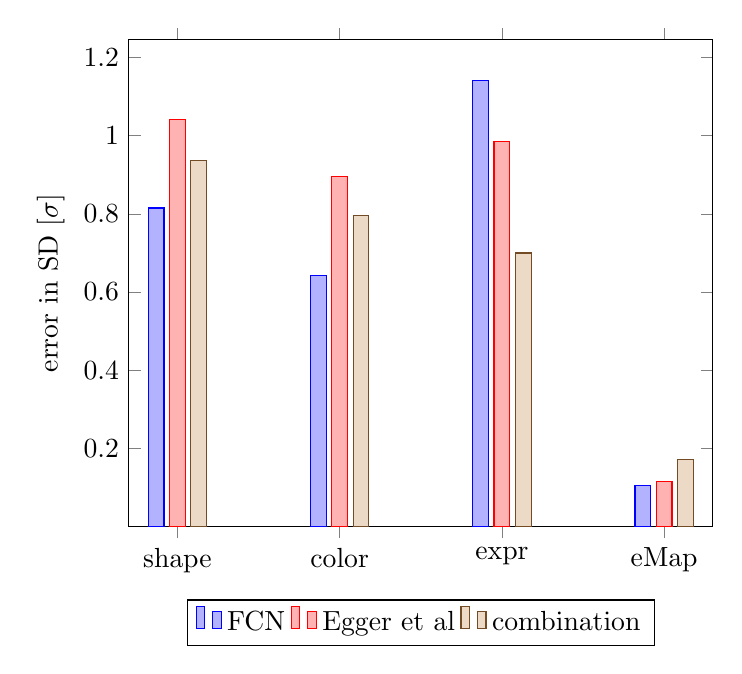
\begin{tikzpicture} 
		\begin{axis}[ 
		ybar,
		bar width=0.2cm,
		enlargelimits=0.1, 
		legend style={at={(0.5,-0.15)}, anchor=north,legend columns=-1}, 
		ylabel={error in SD [$\sigma$]},
		symbolic x coords={shape,color,expr,eMap}, 
		xtick=data,
		%nodes near coords, 
		%nodes near coords align={vertical}, 
		] 
		
		\addplot coordinates {(shape,0.8148) (color,0.6424) (expr,1.1412) (eMap,0.1045)}; 
		\addplot coordinates {(shape,1.0404) (color,0.8947) (expr,0.9855) (eMap,0.1156)}; 
		\addplot coordinates {(shape,0.9369) (color,0.7965) (expr,0.6999) (eMap,0.1715)}; 
		
		\legend{FCN, Egger et al, combination}
		\end{axis} 
		\end{tikzpicture}
		\pgfplotsset{height=7.5cm,width=4cm,compat=1.9}
		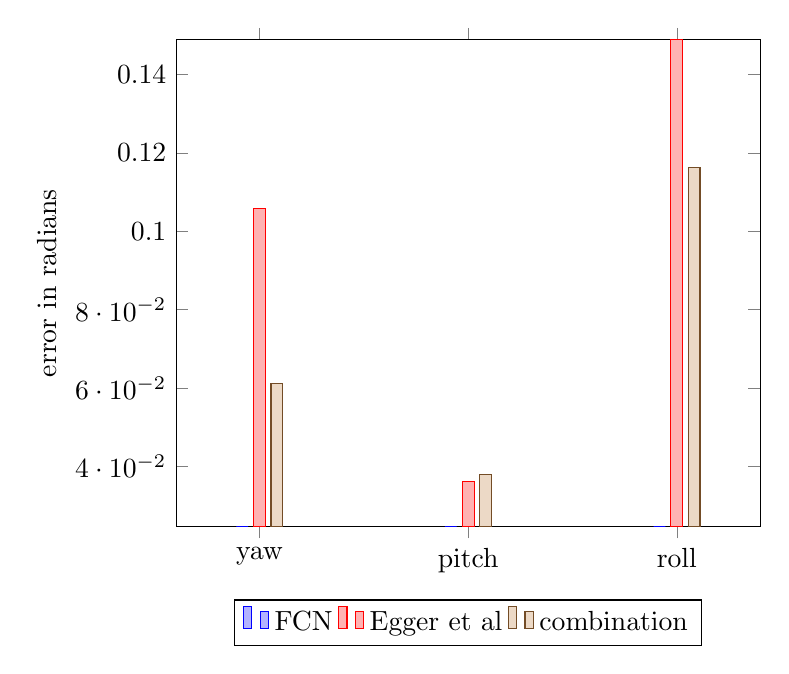
\begin{tikzpicture} 
		\begin{axis}[ 
		ybar,
		bar width=0.15cm,
		%enlarge limits=0.05,
		enlarge y limits=0.00,
		enlarge x limits=0.2,
		legend style={at={(0.5,-0.15)}, anchor=north,legend columns=-1}, 
		ylabel={error in radians},
		symbolic x coords={yaw,pitch,roll}, 
		xtick=data,
		] 
		
		\addplot coordinates {(yaw,0.0247) (pitch,0.0247) (roll,0.0247)}; 
		\addplot coordinates {(yaw,0.1059) (pitch,0.0362) (roll,0.1489)}; 
		\addplot coordinates {(yaw,0.0611) (pitch,0.0379) (roll,0.1163)}; 
		
		\legend{FCN, Egger et al, combination}
		\end{axis} 
		\end{tikzpicture}
	\end{center}
	\caption{A comparison of the Basel Face Model parameters. In this plot, the fits with the masks of Egger, of the FCN [Figure \ref{fig:chap3:zlabelsandfits}], and with the combined mask [\Cref{fig:chap4:bsp1_fit_combined}] are compared. Per parameter, only the first 5 dimensions are considered. In all considered Basel Face Model parameters (shape, color, and expression), the version with the combined mask has a lower error than the slower fit with the mask of Egger et al alone.}
	\label{fig:chap4:fit_comparison_1}
\end{figure}

\begin{figure}
	\centering
	\subbottom[Egger et al]{\includegraphics[width=0.2\textwidth]{Figures/chap4/illuminations/test6_EGGER.png}}
	\subbottom[FCN]{\includegraphics[width=0.2\textwidth]{Figures/chap4/illuminations/test6_FCN.png}}
	\subbottom[combination]{\includegraphics[width=0.2\textwidth]{Figures/chap4/illuminations/test6_combined.png}}
	\subbottom[groundtruth]{\includegraphics[width=0.2\textwidth]{Figures/chap4/illuminations/test6_groundtruth.png}}
	
	\caption{The illuminations of the last example rendered on a sphere. It seems like the illumination with the FCN mask is dull and has no specular term (only ambient). However, the illumination with the combined mask is strongly based on illumination (a).}
	\label{fig:chap4:bsp1_illumination}
\end{figure}
  
\section{Evaluation on the Original Face}
Because we showed in \Cref{sec:Oversegmentation} that the iterative algorithm of Egger et al tends to oversegment and labels skin-parts other than the face, we repeat the experiment with a rendering that shows ears, hairline, and neck too - the 'bfm' version of the Basel Face Model.

\begin{figure}
\centering
\subbottom[initial mask of the FCN]{\includegraphics[width=0.24\textwidth]{Figures/chap3/hands_test0_mask_FCN_.png}\label{fig:chap4:bsp2_mask_FCN}}
\subbottom[segmentation of Egger et al]{\includegraphics[width=0.24\textwidth]{Figures/chap3/hands_test0_mask_EGGER_.png}\label{fig:chap4:bsp2_mask_EGGER}}
\subbottom[combined segmentation]{\includegraphics[width=0.24\textwidth]{Figures/chap4/hands_setting2_test0_mask_combined.png}\label{fig:chap4:bsp2_mask_combined}}
\subbottom[fit with the combined mask (Subfigure (c))]{\includegraphics[width=0.24\textwidth]{Figures/chap4/hands_setting2_test0_fit_combined.png}\label{fig:chap4:bsp2_fit_combined}}
\caption{An example of the combination of the two masks. [Figure \ref{fig:chap4:bsp2_mask_FCN}] shows the segmentation of the FCN while [Figure \ref{fig:chap4:bsp2_mask_EGGER}] shows the segmentation by Egger et al. The combination is depicted in [Figure \ref{fig:chap4:bsp2_mask_combined}]. The target image for this example is the same as in [Figure \ref{fig:chap3:hands_setting2_occluded}]. [Figure \ref{fig:chap4:bsp2_fit_combined}] shows the resulting fit with the combined mask.}
\label{fig:chap4:bsp2}
\end{figure}



\pgfplotsset{height=7.5cm,width=8.5cm,compat=1.9}
\begin{figure}
	\begin{center}
		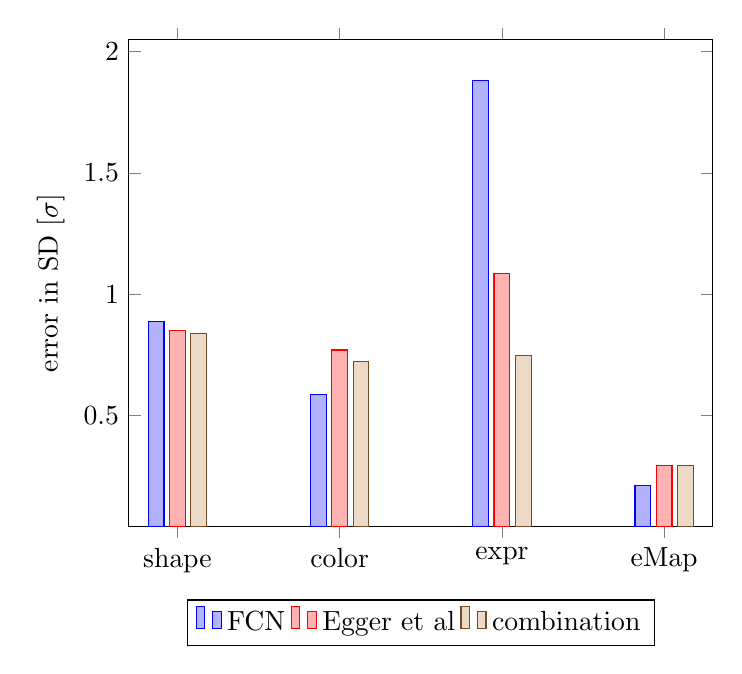
\begin{tikzpicture} 
		\begin{axis}[ 
		ybar,
		bar width=0.2cm,
		enlargelimits=0.1, 
		legend style={at={(0.5,-0.15)}, anchor=north,legend columns=-1}, 
		ylabel={error in SD [$\sigma$]},
		symbolic x coords={shape,color,expr,eMap}, 
		xtick=data,
		%nodes near coords, 
		%nodes near coords align={vertical}, 
		] 
		
		\addplot coordinates {(shape,0.8878) (color,0.5868) (expr,1.8812) (eMap,0.2104)}; 
		\addplot coordinates {(shape,0.8489) (color,0.7704) (expr,1.0859) (eMap,0.2927)}; 
		\addplot coordinates {(shape,0.8397) (color,0.7218) (expr,0.7472) (eMap,0.2927)}; 
		
		\legend{FCN, Egger et al, combination}
		\end{axis} 
		\end{tikzpicture}
		\pgfplotsset{height=7.5cm,width=4cm,compat=1.9}
		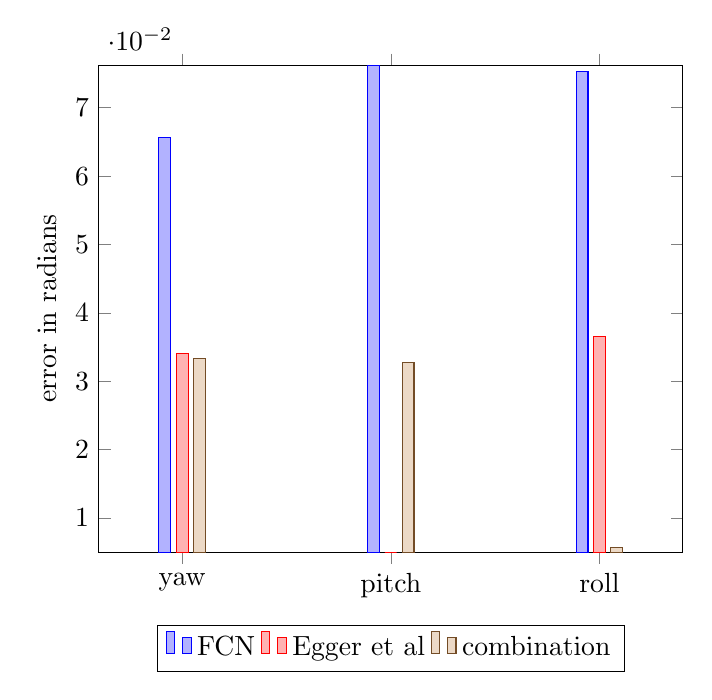
\begin{tikzpicture} 
		\begin{axis}[ 
		ybar,
		bar width=0.15cm,
		%enlarge limits=0.05,
		enlarge y limits=0.00,
		enlarge x limits=0.2,
		legend style={at={(0.5,-0.15)}, anchor=north,legend columns=-1}, 
		ylabel={error in radians},
		symbolic x coords={yaw,pitch,roll}, 
		xtick=data,
		] 
		
		\addplot coordinates {(yaw,0.0657) (pitch,0.0762) (roll,0.0753)}; 
		\addplot coordinates {(yaw,0.0341) (pitch,0.0050) (roll,0.0365)}; 
		\addplot coordinates {(yaw,0.0333) (pitch,0.0327) (roll,0.0057)}; 
		
		\legend{FCN, Egger et al, combination}
		\end{axis} 
		\end{tikzpicture}
	\end{center}
	\caption{A comparison of the Basel Face Model parameters. In this plot, the fits with the masks of Egger, of the FCN [Figure \ref{fig:chap3:zlabelsandfits_setting2}], and the fit with the combined mask [\Cref{fig:chap4:bsp1_fit_combined}] are compared. For each parameter, all dimensions are considered. With the combined segmentation, the fit is a tiny bit better than with the segmentation of Egger et al alone.}
	\label{fig:chap4:fit_comparison_2}
\end{figure}

\begin{figure}
	\centering
	\subbottom[Egger et al]{\includegraphics[width=0.24\textwidth]{Figures/chap4/illuminations/test0_EGGER.png}}
	\subbottom[FCN]{\includegraphics[width=0.24\textwidth]{Figures/chap4/illuminations/test0_FCN.png}}
	\subbottom[combination]{\includegraphics[width=0.24\textwidth]{Figures/chap4/illuminations/test0_combined.png}}
	\subbottom[groundtruth]{\includegraphics[width=0.24\textwidth]{Figures/chap4/illuminations/test0_groundtruth.png}}
	
	\caption{The illuminations of the last example rendered on a sphere. It seems like (as in the previous example) the illumination with the FCN mask is dull and has no specular term (only ambient). Again, the illumination with the combined mask is strongly based on illumination (a).}
	\label{fig:chap4:bsp2_illumination}
\end{figure}



\chapter{Conclusion}
This thesis tested and analysed a fully convolutional network (FCN) for segmenting facial images under occlusion. The used network was trained by Nirkin et al \cite{nirkin2018_faceswap} on a rich and diverse dataset. They claim that the speed and the accuracy of this segmentation method outperforms other approaches that were made especially for this task.\\
\\
We evaluated the segmentation accuracy of the network on two real-life datasets. In one of them, every image was supplied with the ground truth labels, which determine whether a pixel belongs to the face or not. A comparison of both segmentations showed that the segmentation of the FCN contained very few false positives. However, the FCN only recognises about 4/5 of the actual facial region (false negatives). In a further step, the network was evaluated on synthetic images in order to be
in full control of all parameters and to be able to simulate every possible face. The results show that there is a hierarchy among the rotations that determine the orientation of the face. Regardless of whether the face is hidden or not, the FCN is the most vulnerable to large roll rotations, then pitch rotations, and least important are the yaw rotations. That is a strange result because no matter how the face is rolled, the information does not change. We expect that the reason for this is the training of the FCN. 

\begin{figure}
	\centering
	\includegraphics[width=0.5\textwidth]{Figures/chap5/tran_frames.png}
	\caption{Three examples of training images used by Nirkin et al. These are pictures of the recent Janus CS2 dataset by Klare et al \cite{IARPAJanus}. It looks as if the face had not been turned on any of the images in the whole dataset. The first two images are overlaid with synthetic occlusions. The third one depicts the interface used for semi-supervised labeling.}
	\label{fig:chap5:train_images}
\end{figure}

Egger et al \cite{egger_paper} propose an EM-like method to simultaneously segment a face out of a given image and reconstruct it.
We compare the segmentations of Egger et al with the segmentations of the FCN and find that: [1] The approach of Egger et al oversegments the image. [2] The method of Egger et al tends to exclude important details like the eyes due to their strong variability in color and shape. [3] The FCN often fails in recognising and segmenting thin occlusions which is possible with the approach of Egger et al.\\
\\
The runtime of the FCN is much faster compared with the iterative segmentation of Egger et al. On our GPU, the segmentation with the FCN takes approximately 3 seconds, while the algorithm of Egger et al takes 2 minutes (according to the paper \cite{egger_paper} of Egger et al).

\begin{figure}
\centering
\subbottom[original]{\includegraphics[width=0.2\textwidth]{Figures/chap5/harry_original.png}\label{fig:tm:tm1}}
\subbottom[segmentation of Egger et al]{\includegraphics[width=0.2\textwidth]{Figures/chap4/harry_mask_EGGER_.png}\label{fig:tm:tm2}}
\subbottom[segmentation of FCN]{\includegraphics[width=0.2\textwidth]{Figures/chap4/harry_mask_FCN_.png}\label{fig:tm:tm3}}
\caption{Comparison of the two segmentations ((b) and (c)) of the same facial image (a).}
\label{fig:chap5:harry}
\end{figure}

It is difficult to say which mask is better. In order to compare these masks in numbers, both segmentations are used as a mask for fitting synthetic face images, of which we know the correct 3DMM parameters. It turns out that due to the very few false positives of the FCN segmentation, the fit in many cases gets better (in 3DMM parameters) than that with the mask of Egger et al. On the other hand, real facial images are obscured by a variety of objects (not just microphones, hands, and glasses). The method of Egger can recognise these and therefore their mask often leads to better fits on real-world data than with the mask of the FCN [\Cref{appendix:real-world data}].

%Both approaches have their weaknesses and strengths, which we try to combine. Therefore, we take the iterative algorithm of Egger et al and give it the FCN-Segmentation as an initial segmentation. Since this algorithm uses a Metropolis-Hastings method, the final mask looks very similar to Egger et al's mask without the integration.

\section{Future Work}
The Integration in Chapter 4 was not optimal, because the resulting mask came very close to the one estimated by Egger et al itself. Our setting executed the FCN and then let the combined segmentation and fitting algorithm update the mask in all 20 iterations. It would be interesting to see what happens if the algorithm of Egger et al could only improve the initial FCN-Segmentation in a few last iterations. It is strange that the illumination estimation does not improve although an initial segmentation is used for this task (the original approach of egger et al does not use a mask/segmentation to determine the illumination parameters). This is an interesting starting point for further research on how to optimally combine both segmentations.
%\input{./Chapters/Chapter6}
%\input{./Chapters/Chapter7}
%% ----------------------------------------------------------------
\thesisappendix
\thesisbib
\begin{appendices}
	\chapter{Appendix}

\section{COFW-Images and Fits}
\label{appendix:COFW}

\begin{figure}
	\centering
	\includegraphics[width=0.9\textwidth]{Figures/appendix/COFW_Fits_Appendix.png}
	\caption{The additional images of Figure \ref{fig:chap2:COFW_Fits}. In each tuple the first plot shows the fit with the mask of egger et al. and the second plot is made with the segmentation of the FCN.}
	\label{fig:chap2:COFW_Fits_Appendix}
\end{figure}

\vspace{3cm}

\section{Datasets other than Hands(which are shown in the thesis)}
\label{appendix:otherDatasets}

\includepdf[landscape=true,pages={1-16}, angle=180]{Figures/appendix/forAppendix.pdf}

\includegraphics[width=1\textwidth]{Figures/appendix/Real-Life/Real-Life_1.pdf}
\label{appendix:real-world data}
\includegraphics[width=1\textwidth]{Figures/appendix/Real-Life/Real-Life_2.pdf}


\section{Discussion of the Results}
For the synthetic data, a distinction must be made between the occlusions on which the FCN was trained on (hands, micros, glasses) and those unknown to the FCN (random boxes). For known occlusions, the FCN's mask is often more accurate than the one of Egger et al. If these masks are used for fitting, the errors of the parameters ('shape', 'color', 'expression', 'environmentMap') are either very close to those of the fit with the Egger mask, or even better.\\
\\
The random boxes are not recognised by the FCN. The mask is very bad compared to Egger. However, just a few segmented points are enough to get a good fit. Because of the very low false positive rate of the FCN, the fits are comparable to those with the mask of Egger et al. Without occlusion, the masks of the FCN are clearly better than those of Egger. The resulting fits are almost impossible to compare with the naked eye. Due to the Basel Face Model parameters, the fit with the FCN mask is sometimes better than the one with the segmentation of Egger et al.\\
\\
An eye-catching detail is that with the segmentation of Egger et al on the setting with the 'bfm' rendering (on the no occlusion dataset) a very small error of the shape parameter can be achieved. This could be because much more of the face shape is known due to the over-segmentation.

The real life data shows the enormous advantage of Egger. Although the segmentation of the FCN is not bad. The occlusion-aware method of Egger et al can recognise very thin partial coverings such as glasses and separate them from the facial region.


\section{Parametric-Face-Image-Generator}
We extended the Parametric-Face-Image-Generator of Kortylewski et al \cite{parametric}. In our version the option "occlusionMode" in the configuration files can now be set to:
\begin{itemize}[nolistsep]
	\item \textbf{"eyes"}: A circle occludes the picture centered on the pupil centers of the face.
	\item \textbf{"random-1"}: A  hand hides the picture in a random place in a random orientation.
	\item \textbf{"random-2"}: A  microphone hides the picture in a random place in a random orientation.
	\item \textbf{"random"}: A randomly chosen occlusion image hides the picture in a random place.
	\item \textbf{"box"}: A box filled with an arbitrary color hides the image.
	\item \textbf{"box-whiteNoise"}: A box filled with Gaussian white noise hides the image.
	\item \textbf{"box-skinColor"}: Boxes filled with the colour at the tip of the chin hide the image on a random place.
	\item \textbf{"box-[0-100]"}: Boxes filled with a random colour sized that they occlude the specified amount of face pixels.
	\item \textbf{"loop"}: Produces 20 copies of the same image, each with a box occluding 2,4,6,...,40 \% of the face.
	\item \textbf{"texture"}: Fills a randomly placed box with a specified texture image.% specified in the folder 'textures'.
\end{itemize}


\begin{figure}
	\hspace*{\fill}%
	\subbottom[A facial image of the parametric face image generator with all landmarks activated.]{\includegraphics[width=0.3\textwidth]{Figures/chap3/original_all_lms.png}}\hfill
	\subbottom[The same image as in (a) but with an occlusion and two underlying landmarks which are disabled because they're not visible anymore.]{\includegraphics[width=0.3\textwidth]{Figures/chap3/occluded_parts_lms.png}}
	\hspace*{\fill}%
	\caption{Because of the occlusion, certain landmarks had to be disabled. The image shows original landmarks (green dots) and the landmark which had to be deactivated (red dots).}
	\label{appendix:lms}
\end{figure}

The software provides csv-files, rps-files, tlms-files, ground truth masks, images with occlusions and images without occlusions for both the 'bfm' version and for the tailored 'face12' version of the Basel Face Model. If an occlusion gets rendered over a landmark, it gets disabled. 
\end{appendices}
%% ----------------------------------------------------------------
\thesisback
\input{./Back/DeclarationOfAuthorship}
%% ----------------------------------------------------------------
\end{document}
%% ----------------------------------------------------------------
